% !TEX spellcheck = en_US
%=================================================================================
\chapter{Controller design objectives}
%=================================================================================
\section{Advanced Controller}

Wind turbine use closed-loop control systems to continuously adjust their operations based on feedback. Figure 1, illustrates the advanced control closed-loop diagram of a wind turbine. 
\\[16pt]
The torque controller optimizes power production below rated speed and maintain rated power and maintain rated power above rated wind speed by adjusting generator torque $(M_G)$ based on generator speed $(\Omega_G)$. Advance torque control uses a PI controller with anti-windup to regulate the generator torque based on the difference between the actual and reference generator speeds. Above rated wind speed, Pitch controller maintains the rated generator speed $(\Omega_{G,rated})$ by adjusting blade pitch angle $(\theta)$, which ensures the rated power is maintained. With increasing wind speed, the pitch angle increases to reduce power coefficient $(c_p)$. Once the wind speed reaches the rated value, the generator torque is maintained at its rated value. The control is categorized into different regions, as detailed in Section 2.2.

\begin{figure}[htbp]
	\centering
	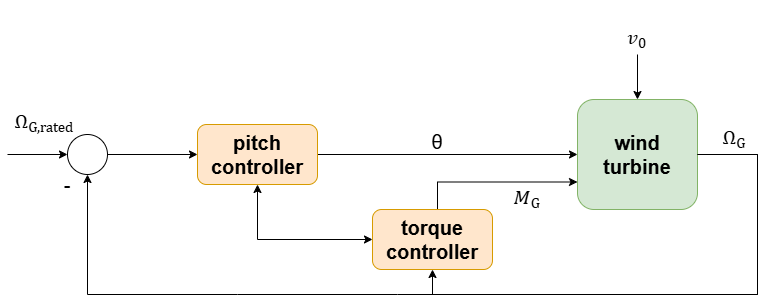
\includegraphics[width=\textwidth]{Figure/Figure_1.png}
	\caption{Advance Wind Turbine Controller}
\end{figure}
 

\section{Control Region Soni}

\section{Generator Torque controller Soni}

\section{Collective pitch controller CPC Julius}

\section{Tower Damper Felix}